\section{\cyclus}
\label{sec:cyclus}
\cyclus is an agent-based \gls{nfc} simulator that is versatile, open source,
and modular. The software achieves this versatility through a series of generic
archetypes that are primarily transaction-based. Over the years, the user
community and developers have created a litany of nuclear-specific archetypes
for everything from proliferation assessment to fuel burnup. Many standard fuel
cycle facilities have been implemented in the \cycamore repository
\cite{Carlsen_cycamore_2014}, which holds technology-agnostic archetypes for
material sources, material sinks, enrichment services, separations
capabilities, and a generic reactor.

\cyclus treats each facility as an agent that can interact with other agents in
the simulation. The agents are defined by their capabilities and the resources
they can provide or consume. The agents are connected through a market
mechanism called the \gls{dre} that allows agents to make requests for
resources and respond to requests from other agents, this is a unique feature
of \cyclus. The \gls{dre} is a key component of the \cyclus simulation
framework that allows for the dynamic exchange of resources between agents. The
\gls{dre} is responsible for matching resource requests with offers from
suppliers and ensuring that the resources are exchanged fairly and efficiently.

Materials, or commodities in the parlance of the \cyclus ecosystem, are passed
by agents through the \gls{dre} in recorded transactions. A commodity can be
anything, from raw materials like uranium ore to contextual concepts (e.g.,
money, permits, emissions, or social acceptance). The transactions are recorded
in a database that can be queried to determine the flow of materials through
the simulation. As Huff et al. outline in their 2016 paper
\cite{huff_cyclus_intro_2016}, treating facilities and materials allows for
flexibility in the level of fidelity for each.

% discuss recipes
As \cyclus is a transactions code and not necessarily a physics code,
the reactors incorporate reactor physics through pre-defined "recipes,"
where the user specifies the isotopic concentration of the fresh and
used fuel. Pre-defining recipes also reduces the precision with which
fuel compositions are calculated. For example, depending on how fuel is
discharged from a core at the end of a reactor's lifetime, there are
instances when the model will over or under-predict the concentration of
important isotopes; thereby throwing off calculations. Users approximate
the burnup of each fuel element with the same input recipe to be the
same; however, in this work we incorporate a cascading enrichment from
\gls{leu+} to \gls{haleu} as some advanced reactor companies have
redesigned their cores to make use of both; \gls{leu+} in the short term,
while they work with the government to establish the supply chain for
\gls{haleu}.

% discuss EVER and CLOVER?
% Novel in this work is our use of a low fidelity archetype based on the \cycamore reactor \gls{ever}, which allows the user to specify multiple recipes for the fuel and change between them at specific times.

% discuss region, institution, and facility relationships
In \cyclus, the user defines the simulation by specifying the regions,
institutions, and facilities that will be present in the simulation. Regions
are collections of institutions, and institutions are collections of facilities
(facilities are the agents interacting in the simulation). The user can define
the relationships between regions, institutions, and facilities to model the
flow of materials and resources through the simulation. Through initial
conditions, the user can tailor their simulation for any historical or imagined
starting point based on the expected facilities and resources available from
the outset.

\subsection{Fuel Depletion}
\label{sec:depletion}

Fuel depletion is a critical aspect of fuel cycle simulations, as it directly
influences the characteristics and behavior of \gls{uf}. The composition of
this fuel, shaped by factors like decay heat, the quantity of fissile material,
and the volume of \gls{uf}, has profound implications for various stages of the
nuclear fuel cycle. The effects of depletion on these properties are
significant: they not only impact the thermal and physical characteristics of
the fuel but also affect practical considerations such as the transportation of
\gls{uf}, the limits of repository storage, and the potential for reprocessing
and recycling of materials. Thus, any comprehensive fuel cycle simulation must
account for fuel depletion, ensuring that the resulting data reflects realistic
conditions and constraints.

In many fuel cycle simulators, fuel depletion is managed using pre-defined
compositions, which allow for rapid calculations and straightforward modeling
of fuel cycles. Tools such as VISION \cite{yacout_visionverifiable_2006}, the
CYCAMORE Reactor archetype in \cyclus--which uses the aforementioned
"recipes"--, and ORION utilize this methodology. In these frameworks, the
compositions of \gls{uf} are established in advance, often derived from
separate depletion modeling efforts. This approach is particularly effective
for once-through fuel cycles, where fresh fuel compositions remain constant
across refueling periods, leading to minimal variation in the characteristics
of discharged fuel. While this method offers simplicity and speed, it may not
capture the nuanced behaviors seen in more complex fuel cycles, where dynamic
changes in fuel composition are more pronounced.

To further enrich the capabilities of \cyclus in modeling fuel depletion,
several archetypes have been developed. Bright-lite
\cite{schneider_integrated_2016}, for instance, introduces a comprehensive
framework for evaluating fuel compositions based on burnup and criticality.
This archetype offers two operational modes—forward and blending mode—allowing
users to tailor depletion modeling to specific scenarios. In forward mode, the
initial recipe is depleted based on a given fluence. In blending mode, the
reactor is connected to a fabrication facility that mixes material streams to
meet a burnup criticality or conversion ratio. The burnups and material
definitions need to be given, which is the first step in implementing this
archetype. CyBORG \cite{skutnik_cyborg_2016}, another notable archetype,
integrates \cyclus with ORIGEN by generating a problem-specific cross section
library (which it then feeds to ORIGEN to perform a single depletion
calculation for the core), enabling a more nuanced approach to modeling fuel
cycles. Although CyBORG requires access to the export-controlled ORIGEN, it
significantly enhances the accuracy of \gls{uf} compositions. Additionally, the
ann\_pwr \cite{bae_deep_2020} archetype employs neural networks trained on
historical data to predict fuel compositions based on burnup and initial
enrichment. While achieving results with less than 1\% error in 0.23\% of the
time as ORIGEN, ann\_pwr's applicability is limited to \gls{pwr} designs
currently, highlighting a need for broader models that can encompass diverse
reactor types.

Dynamic modeling of fuel depletion represents an evolution in fuel cycle
simulations, allowing for real-time updates to fuel compositions as they change
throughout the cycle. This approach is crucial for accurately reflecting the
influences of fuel depletion on material properties. Various simulators outside
the \cyclus ecosystem, including ORION \cite{feng_standardized_2016}, DYMOND
\cite{richards_application_2021}, and NFCSim \cite{schneider_nfcsim_2005},
offer capabilities for dynamic modeling. For instance, ORION allows users to
define material compositions using recipes or can autonomously model decay and
depletion. DYMOND enhances accuracy by coupling with ORIGEN2, enabling
criticality searches that refine fresh fuel compositions based on updated
\gls{uf} data. NFCSim's coupling with the \gls{lace} further exemplifies this
trend by employing fluence-dependent calculations to ascertain the evolving
nature of nuclear materials. These advancements in dynamic modeling are
essential for improving the fidelity and reliability of fuel cycle simulations,
particularly as the nuclear industry moves toward more intricate and
sustainable fuel management strategies.

The OpenMCyclus archetype \cite{openmcyclus_paper} enhances the \cyclus
ecosystem by introducing an open-source real-time fuel depletion tool for
\cyclus simulations. Unlike traditional approaches that rely on pre-defined
recipes for fuel compositions, OpenMCyclus integrates with OpenMC
\cite{romano_openmc_2015} to dynamically update spent fuel compositions
throughout the simulation, allowing for greater accuracy and flexibility in
modeling various reactor designs. This real-time depletion capability is
valuable for assessing the impacts of different fuel cycle strategies, as it
accommodates changes in fuel composition and operational conditions without the
need for restrictive licensing agreements associated with other depletion tools.

\subsection{Archetypes and Time Management}
\label{sec:archetypes_and_time_management}

Throughout the \cyclus ecosystem, archetypes interact with the \gls{dre} and
each other in a fixed, user-defined, time step, forcing the entire simulation
to operate on the smallest universal time step. For example, if a fabrication
facility can produce material every 2 months but the enrichment facility can
only provide material every 3 months, we would need to use a 1-month time step
to capture both. When the time step is smaller than the minimum for a given
facility, that facility still participates in the \gls{dre} with a zero bid.
These zero bids, across hundreds of facilities, add complexity and
inefficiencies to solving the transaction problem at each time step.

Examining the \cyclus ecosystem, we identified an archetype called PatternSink
wherein the user can alter the frequency that the material sink, often called
the repository, can accept the material. We have created an example of this
archetype with a simple A-B-C scenario, shown in Figure \ref{fig:a-b-c}. In
this scenario, material is received from a source (A) to a reactor (B) with a
final (C) sink that can only accept material at a certain frequency.

\begin{figure}[!ht]
    \centering
    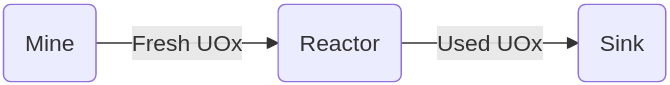
\includegraphics[scale=0.4]{images/cyclus/a-b-c.png}
    \caption{Simple A-B-C Scenario}
    \label{fig:a-b-c}
\end{figure}

If we track the material being received by the sink it becomes clear that this
frequency alters how frequently the archetype updates its internal
understanding of time. It appears in Figure \ref{fig:pattern_freq_50} as though
multiple groups of material are received in one time step despite this
archetype not having an idea of individual shipments. The way this archetype
accomplishes the artificial restriction on accepting material is by simply not
updating the time step that the archetype is at until the next universal time
step is met. Regardless of function, this is the only example of the
flexibility of timestep we found in the ecosystem.

\begin{figure}[!ht]
    \centering
    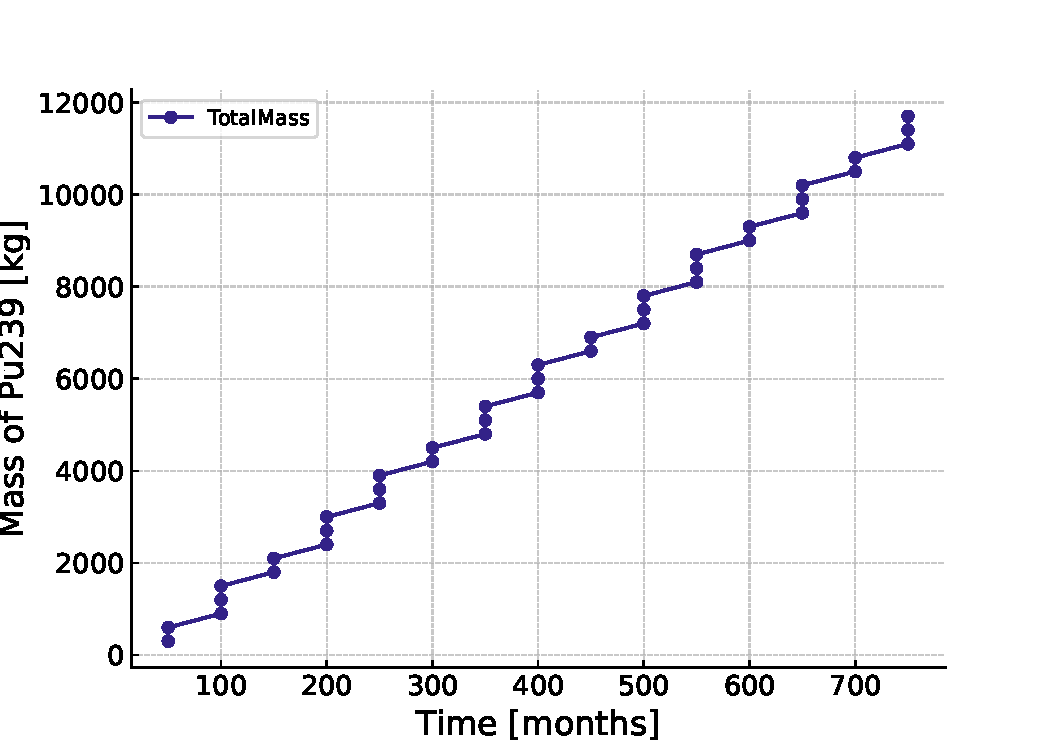
\includegraphics[scale=0.75]{images/cyclus/pattern_sink_fuel_transactions.pdf}
    \caption{Acceptance of $^{239}$Pu into the sink with a frequency of 50 months}
    \label{fig:pattern_freq_50}
\end{figure}

While archetypes like PatternSink introduce new, internal capabilities, they
all inherit a set of base capabilities from the \cyclus toolkit. In this work,
we implement a fundamental toolkit capability that any archetype in the \cyclus
ecosystem can use with one implementation. The \cyclus toolkit provides a
modular and extensible framework for modeling \glspl{nfc}, allowing users to
create custom archetypes that simulate various facilities and processes. These
base capabilities standardize how archetypes create material buffers, interact
with the \gls{dre}, and connect to the internal clock of the simulation, which
are essential for coordinating the agents and commodities across their complex
interactions within a \gls{nfc}. Additionally, the toolkit includes features
such as dynamic resource allocation, customizable agent behaviors, and detailed
tracking of material flows, which are crucial for simulating the lifecycle of
nuclear materials.

The toolkit's modular architecture allows for the seamless integration of new
archetypes and models, promoting innovation and collaboration within the
\cyclus community. We aim to provide the most versatile and powerful foundation
for \cyclus users by focusing on these core toolkit capabilities. This will
enable researchers and developers to create more accurate and detailed
simulations of \glspl{nfc}, ultimately allowing for better decision-making and
policy development in the nuclear industry. We have identified the appropriate
policy to update in material transactions and leverage the existing dormant
purchasing policy to create a robust implementation in the \cycamore
archetypes, ensuring that the most users possible will benefit. By implementing
these improvements, we aim to ensure that the \cyclus toolkit remains at the
forefront of \gls{nfc} simulation, providing a robust and flexible platform for
users to explore and analyze various scenarios and strategies.